\documentclass[spanish]{article}

\usepackage{arxiv}

\usepackage[utf8]{inputenc} % allow utf-8 input
\usepackage[T1]{fontenc}    % use 8-bit T1 fonts
\usepackage{lmodern}        % https://github.com/rstudio/rticles/issues/343
\usepackage{hyperref}       % hyperlinks
\usepackage{url}            % simple URL typesetting
\usepackage{booktabs}       % professional-quality tables
\usepackage{amsfonts}       % blackboard math symbols
\usepackage{nicefrac}       % compact symbols for 1/2, etc.
\usepackage{microtype}      % microtypography
\usepackage{graphicx}

\title{Site Planning for a Network of Government-operated Weather
Stations in the Dominican Republic Using Zonal Statistics from
Geospatial Sources, Multi-Criteria Decision-Making, and Neighborhood
Analysis}

\author{
    \parbox[t]{10cm}{\centering José-Ramón Martínez-Batlle \\ \orcidlink{0000-0001-9924-0327}}
   \\
    Facultad de Ciencias \\
    Universidad Autónoma de Santo Domingo (UASD) \\
  Santo Domingo, República Dominicana \\
  \texttt{\href{mailto:joseramon@geografiafisica.org}{\nolinkurl{joseramon@geografiafisica.org}}} \\
   \And
    \parbox[t]{10cm}{\centering Michela Izzo Gioiosa \\ \orcidlink{0000-0003-4835-3967}}
   \\
    Directora Ejecutiva \\
    Guakia Ambiente \\
  Santo Domingo, República Dominicana \\
  \texttt{\href{mailto:michela.izzo@guakiambiente.org}{\nolinkurl{michela.izzo@guakiambiente.org}}} \\
  }


% tightlist command for lists without linebreak
\providecommand{\tightlist}{%
  \setlength{\itemsep}{0pt}\setlength{\parskip}{0pt}}


% Pandoc citation processing
\newlength{\cslhangindent}
\setlength{\cslhangindent}{1.5em}
\newlength{\csllabelwidth}
\setlength{\csllabelwidth}{3em}
\newlength{\cslentryspacingunit} % times entry-spacing
\setlength{\cslentryspacingunit}{\parskip}
% for Pandoc 2.8 to 2.10.1
\newenvironment{cslreferences}%
  {}%
  {\par}
% For Pandoc 2.11+
\newenvironment{CSLReferences}[2] % #1 hanging-ident, #2 entry spacing
 {% don't indent paragraphs
  \setlength{\parindent}{0pt}
  % turn on hanging indent if param 1 is 1
  \ifodd #1
  \let\oldpar\par
  \def\par{\hangindent=\cslhangindent\oldpar}
  \fi
  % set entry spacing
  \setlength{\parskip}{#2\cslentryspacingunit}
 }%
 {}
\usepackage{calc}
\newcommand{\CSLBlock}[1]{#1\hfill\break}
\newcommand{\CSLLeftMargin}[1]{\parbox[t]{\csllabelwidth}{#1}}
\newcommand{\CSLRightInline}[1]{\parbox[t]{\linewidth - \csllabelwidth}{#1}\break}
\newcommand{\CSLIndent}[1]{\hspace{\cslhangindent}#1}

\usepackage[utf8]{inputenc} \usepackage[T1]{fontenc} \usepackage{orcidlink} \usepackage{float} \usepackage[all]{nowidow} \usepackage{xcolor} \usepackage{tabu} \setlength{\defaultaddspace}{0pt} \renewcommand{\arraystretch}{1.5} \newcommand{\beginsupplement}{ \setcounter{table}{0} \renewcommand{\thetable}{S\arabic{table}} \renewcommand\tablename{Tabla} \setcounter{figure}{0} \renewcommand{\thefigure}{S\arabic{figure}} \renewcommand\figurename{Figura} } \usepackage[hidelinks]{hyperref} \usepackage{xurl} \usepackage[left]{lineno} \linenumbers
\usepackage{booktabs}
\usepackage{longtable}
\usepackage{array}
\usepackage{multirow}
\usepackage{wrapfig}
\usepackage{float}
\usepackage{colortbl}
\usepackage{pdflscape}
\usepackage{tabu}
\usepackage{threeparttable}
\usepackage{threeparttablex}
\usepackage[normalem]{ulem}
\usepackage{makecell}
\usepackage{xcolor}
\begin{document}
\maketitle



%\newpage

\begin{abstract}
Many weather station networks lack sufficient representativeness, and
their station density is often inadequate to capture spatial and
climatic variability effectively. Optimal site selection is therefore
essential to enhance spatial coverage and improve data quality. This
study proposes a methodology for identifying optimal sites for a
meteorological station network in the Dominican Republic, utilizing a
multi-criteria decision-making framework based on the Analytic Hierarchy
Process (AHP) and neighborhood analysis. Using the H3 library as a
spatial indexing tool, zonal statistics were derived from geospatial
variables, including seasonality, habitat heterogeneity, proximity to
water bodies, slope, solar radiation, and elevation. Expert-defined
weights were assigned to each variable based on their relative
importance. Areas with high topographic and climatic variability were
prioritized to maximize spatial representativeness. Results highlight
thermal and precipitation seasonality, elevation, and solar radiation as
the most influential variables, emphasizing the need to collect data in
elevated areas with marked seasonality. Sites were evenly distributed
across three density scenarios, ensuring robust climatic and topographic
coverage while avoiding redundancy through proximity constraints to
existing stations. The proposed network would provide essential data for
meteorological and climatic research in the region. Future studies
should assess the accessibility and feasibility of the selected sites
and incorporate additional environmental variables into the framework.
\end{abstract}

\keywords{
    Weather stations networks
   \and
    Optimal site selection
   \and
    Spatial coverage
   \and
    Multi-criteria decision-making
   \and
    AHP
  }

\hypertarget{introduction}{%
\section{Introduction}\label{introduction}}

Weather stations (WS) are essential for collecting accurate and
up-to-date data on weather and climate in specific regions. The
applications of the data collected by WS extend beyond meteorology and
climatology, finding widespread use in fields such as engineering,
agriculture, urban planning, and geography, among others (Chung et al.,
2018; Marchi et al., 2019; Wilgen et al., 2016; World Meteorological
Organization (WMO) \& The International Association of Hydrological
Sciences, 1976). The data provided by these stations are instrumental in
predicting extreme weather events, such as tropical storms, hurricanes,
tornadoes, and droughts, enabling communities to prepare and respond
effectively. Furthermore, WS data underpin numerous scientific studies
on climate and climate change, helping to better understand atmospheric
dynamics and their impacts on the planet, ultimately contributing to
more informed and effective planning strategies (World Meteorological
Organization (WMO), 1996, 2017a, 2017b).

A robust WS network is crucial for making informed decisions across
various domains and is fundamental for the well-being and safety of
communities and the environment. Planning an adequate WS network is
essential for effective land management. Previous studies, including
those conducted in the Dominican Republic, reveal significant gaps in WS
coverage in key areas and highlight the uneven spatial distribution and
low density of existing networks, which likely affect the accuracy of
collected data (Frei, 2003; Programa Mundial de Alimentos (PMA), 2019;
Rojas Briceño et al., 2021; Theochari et al., 2021).

Many countries have evaluated the design of their WS networks, sometimes
revisiting and improving them multiple times, often with successful
implementations (Frei, 2003). Some have developed site selection
protocols that align with general World Meteorological Organization
(WMO) standards, adapting or extending them to meet the specific needs
of their territories and intended applications (Rojas Briceño et al.,
2021; Theochari et al., 2021).

The Dominican Republic, an island nation in the Caribbean occupying the
eastern two-thirds of Hispaniola, is characterized by its diverse
geography, including coastal plains, mountain ranges, and a tropical
climate. This geographical diversity, combined with its socioeconomic
challenges, makes the country highly vulnerable to the impacts of
climate change, and an insufficient WS network exacerbates this
vulnerability (Izzo et al., 2010; Lincoln Lenderking et al., 2020;
Lohmann, 2016; Mackay \& Spencer, 2017; Ngoc Le, 2019; Roson, 2013).
Improving and expanding the WS network requires investment in technology
and infrastructure, as well as partnerships among government agencies,
private entities, and research institutions (Programa Mundial de
Alimentos (PMA), 2019). However, to optimize the use of limited
resources, it is critical to design, evaluate, and select network
alternatives using weighted criteria.

Research on the design of weather station networks consistently
identifies multi-criteria decision-making (MCDM) methods as ideal for
this purpose (Köksalan et al., 2011; Taherdoost \& Madanchian, 2023;
Thiriez \& Zionts, 1975). These methods leverage geospatial data and
include public input spatially integrated into decision-making using
Geographic Information Systems (GIS) (Chakhar \& Mousseau, 2008; Eastman
et al., 1998; Malczewski, 2004; Rojas Briceño et al., 2021;
Tekleyohannes et al., 2021; Theochari et al., 2021). Studies have
demonstrated the effectiveness of traditional geostatistical techniques
(Ali \& Othman, 2018; Valipour et al., 2019), contemporary deep learning
algorithms in combination with traditional methods (Safavi et al.,
2021), and entropy-based approaches (Bertini et al., 2021). Combining
geospatial data (e.g., GIS and remote sensing) with multi-criteria
analysis (MCA) that assigns relative weights to geographical criteria is
particularly efficient for analyzing diverse variables (Rojas Briceño et
al., 2021).

The Analytic Hierarchy Process (AHP), a well-established multi-criteria
decision-making (MCDM) method, is widely used due to its simplicity, its
ability to provide insights into the analyzed attributes, and its
structured framework for incorporating expert input (Rojas Briceño et
al., 2021). Developed by Thomas Saaty in the 1970s (Saaty, 1977) and
refined in subsequent decades (Saaty, 2001; Saaty \& Tran, 2007), AHP is
used to make decisions involving multiple criteria and alternatives.
Traditionally applied in engineering, social sciences, economics, and
business, AHP has recently been utilized effectively for selecting
optimal WS sites in Peru (Rojas Briceño et al., 2021). AHP involves
breaking down a complex problem into a hierarchical structure of
criteria and subcriteria, followed by pairwise comparisons to assign
relative importance (Saaty \& Tran, 2007). The process includes
identifying objectives and criteria, structuring them hierarchically,
conducting pairwise comparisons, calculating priority values for
criteria, and ranking alternatives based on aggregated priorities.

In this study, we integrate the Analytical Hierarchy Process (AHP) with
geospatial and expert-driven data to systematically identify optimal
sites for meteorological and climatic stations in the Dominican
Republic. We prioritize key environmental and accessibility criteria to
maximize spatial and resource efficiency while minimizing redundancy in
existing networks. Additionally, we propose actionable scenarios for
network expansion that align with international standards, offering
solutions to address data gaps in poorly covered regions. Through this
research, we advance geospatial methodologies and decision-support
frameworks for meteorological infrastructure planning, with potential
applications in broader climatological and environmental sciences.

\hypertarget{materials-and-methods}{%
\section{Materials and Methods}\label{materials-and-methods}}

We applied a sequence of four interdependent steps to develop
alternative designs for weather station (WS) networks, emphasizing the
multi-criteria selection of sites prioritized for their deployment.
First, we gathered data on the existing WS network through consultations
(via forms and visits) with government agencies, including the Dominican
National Meteorological Office (ONAMET, now the Dominican Institute of
Meteorology, INDOMET) and the National Institute of Hydraulic Resources
(INDRHI). These forms were created and managed using the Open Data Kit
(ODK) platform (Get ODK Inc., 2024; Hartung et al., 2010). We also
consulted private entities managing WS networks. These efforts resulted
in consolidated information on station locations, operational status,
and other relevant attributes. This step ensured that the analysis was
grounded in an accurate and comprehensive understanding of the current
state of the WS network.

Subsequently, we implemented an Analytic Hierarchy Process (AHP) to
select the optimal option among different alternatives using selection
criteria weighted by individuals with expertise in the problem (Saaty,
2013). The selected criteria were distance to access routes, thermal
seasonality, rainfall seasonality, habitat heterogeneity, distance to
water bodies, slope, hours of direct sunshine, elevation. These eight
criteria were chosen based on their relevance to the problem, supported
by our expertise as well as previous studies and recommendations from
the World Meteorological Organization (Rojas Briceño et al., 2021; World
Meteorological Organization (WMO) \& The International Association of
Hydrological Sciences, 1976).

We explicitly requested expert consultations, asking respondents to
complete questionnaires electronically. After collecting the responses,
we organized and recoded the data, then evaluated their consistency. We
used only consistent responses to establish the criteria weights, which
were subsequently applied to the available geographic information
sources, including approximately
\href{https://geofis.github.io/zonal-statistics/README.html}{13,000
hexagons containing the corresponding multi-criteria information
distributed across the Dominican Republic} (Martínez-Batlle, 2022).
Afterwards, we created these hexagons using the H3 spatial index library
from Uber and computed zonal statistics with Google Earth Engine (GEE)
(Gorelick et al., 2017; Uber Technologies, Inc., 2024). Specifically, we
employed the GEE Python API to process the data programmatically, using
packages like \texttt{geemap} for map visualization and data handling
(Google Earth Engine Contributors, 2023; Wu, 2020). Finally, we assigned
each hexagon an aggregated priority category, choosing from four
possible options: marginally prioritized, moderately prioritized,
prioritized and essential.

We designed the questionnaires, processed the responses, and weighted
the criteria of geographic information sources using programming
languages. These tasks were performed in the R statistical programming
environment with the following packages: \texttt{ahpsurvey},
\texttt{sf}, \texttt{raster}, \texttt{terra}, \texttt{ggplot2},
\texttt{tidyverse}, \texttt{kableExtra}, \texttt{spdep}, \texttt{units},
\texttt{knitr}, and \texttt{rmarkdown} (Cho, 2019; Hijmans, 2023, 2024;
Pebesma et al., 2016; Pebesma, 2018; Pebesma \& Bivand, 2023; R Core
Team, 2024; Wickham et al., 2019; Xie, 2014; Xie et al., 2020; Zhu,
2021). We also used Python to automate the design of questionnaires and
their integration with Google Forms via its API.

Subsequently, we used the AHP results as input for a constraint-based
exclusion process. In this step, we carefully analyzed the hexagons to
identify those located in areas where accessibility was limited or where
proximity to water bodies posed challenges. Hexagons situated near or
within water bodies were deemed unsuitable for hosting meteorological
stations and were excluded from further consideration. This process
ensured that only feasible locations remained for the next steps of the
analysis.

Finally, to optimize the spatial distribution of weather stations, we
developed a custom site selection function based on neighborhood
analysis. This function generated proposed station locations for three
density scenarios: 100, 150, and 250~km\textsuperscript{2} per station,
aligning with the station density criteria recommended by the World
Meteorological Organization (World Meteorological Organization (WMO),
2020; World Meteorological Organization (WMO) \& The International
Association of Hydrological Sciences, 1976). The algorithm employed
convex hulls and distance maximization to iteratively select points that
were maximally distant from previously chosen locations, ensuring
spatial homogeneity across the coverage area. For each scenario, the
coverage area was defined as the set of hexagons meeting the priority
categories essential or prioritized.

To refine the proposed locations, we incorporated a neighborhood
analysis that utilized continuous distance surfaces (e.g., rasters).
This analysis identified and excluded proposed stations located too
close to existing stations with ``Good or Active'' status in the INDRHI
or ONAMET networks. By doing so, we avoided redundancy and ensured that
the proposed distributions complemented the existing station networks
while maintaining an optimal spatial configuration.

\hypertarget{results}{%
\section{Results}\label{results}}

The operational status and distribution of weather stations (WS) in 2022
reveal key differences between the networks managed by the Dominican
Institute of Meteorology (INDOMET) and the National Institute of
Hydraulic Resources (INDRHI). We analyzed these differences to identify
coverage gaps and opportunities for improvement
(Table~\ref{tab:summaryindometindrhi}). We found that INDOMET operates
87 WS, classifying 36 as ``Active or Good'' (41\%), 51 as ``Inactive or
Not Reported'' (59\%), and none as ``Recoverable.'' In contrast, we
observed that INDRHI's network comprises 54 stations, with 16 classified
as ``Active or Good'' (30\%), 28 as ``Inactive or Not Reported'' (52\%),
and 10 as ``Recoverable'' (18\%). Together, both networks include 141
stations, with 52 in ``Active or Good'' condition, representing 37\% of
the total. Considering only WS classified as ``Active or Good,'' the
spatial representativeness of INDOMET's network corresponds to one
station per 1346~km\textsuperscript{2}, while for INDRHI's network, it
corresponds to one station per 3028~km\textsuperscript{2}.

\begin{figure}[!ht]

{\centering 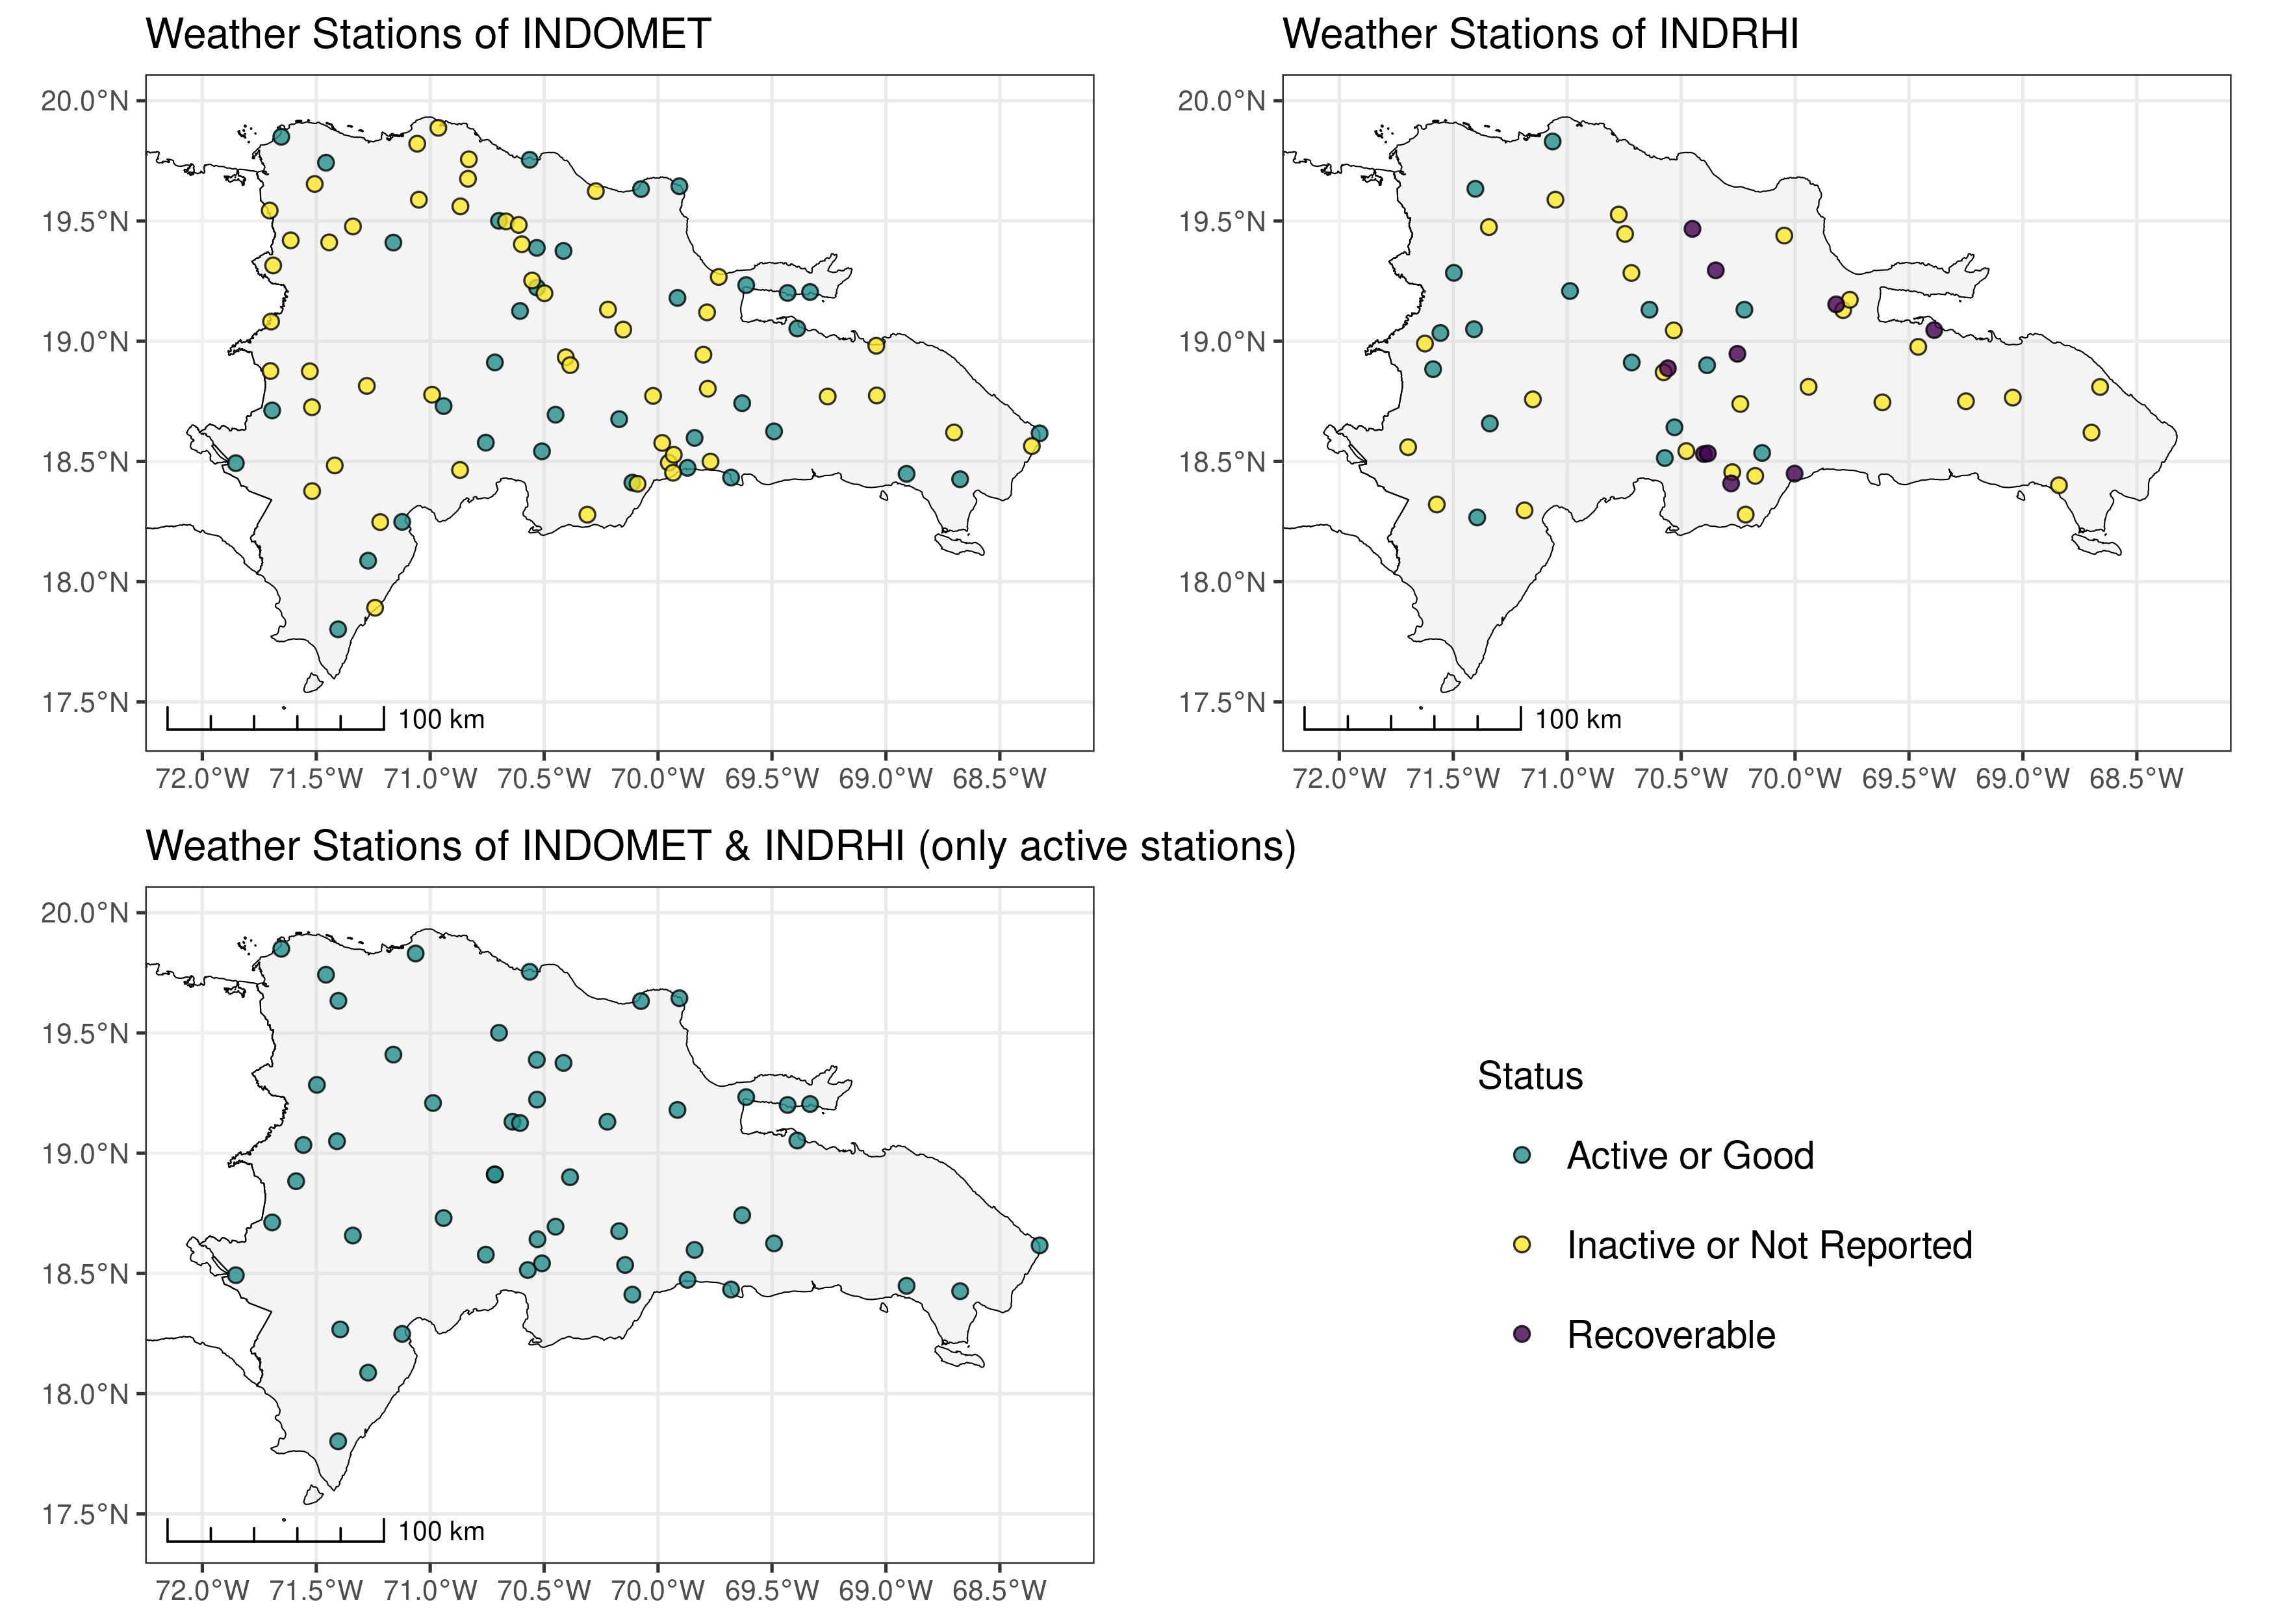
\includegraphics[width=1\linewidth]{figuras/ws_network_2022_grid2} 

}

\caption{Weather station networks in the Dominican Republic for 2022, presented by operational status and management entities. The top two maps show stations managed by the Dominican Institute of Meteorology (INDOMET) and the National Institute of Hydraulic Resources (INDRHI), respectively, categorized as "Active or Good," "Recoverable," or "Inactive or Not Reported." The bottom map consolidates active stations from both institutions to emphasize their combined geographic coverage.}\label{fig:ws_network_2022_grid2}
\end{figure}

We also analyzed the geographic distribution of WS, as shown in
Figure~\ref{fig:ws_network_2022_grid2}, and observed that INDOMET's
network provides broader coverage. We identified that a moderate
proportion of INDRHI's stations could be restored to full operational
status with minimal recovery efforts. By combining the ``Active or
Good'' WS from INDOMET and INDRHI, we also created a map that offers a
comprehensive view of the functional coverage across the Dominican
Republic. This map highlights critical gaps in the spatial distribution
of WS and emphasizes the need to enhance monitoring in underserved areas
to ensure representative weather and climate data coverage.

\begin{table}

\caption{\label{tab:summaryindometindrhi}Summary of weather station status in 2022 by owner (INDOMET and INDRHI) in the Dominican Republic for 2022, including the number of active or good, inactive or not reported, and recoverable stations, along with their total counts}
\centering
\begin{tabular}[t]{lrrrr}
\toprule
\textbf{Owner} & \textbf{Active or Good} & \textbf{Inactive or Not Reported} & \textbf{Recoverable} & \textbf{Total}\\
\midrule
INDOMET & 36 & 51 & 0 & 87\\
INDRHI & 16 & 28 & 10 & 54\\
Total & 52 & 79 & 10 & 141\\
\bottomrule
\end{tabular}
\end{table}

We used the Analytical Hierarchy Process (AHP) to provide a structured
framework for prioritizing criteria and identifying optimal sites for
weather stations, ensuring an objective and expert-driven selection
process. From the eight preselected criteria evaluated by experts, the
four with the highest aggregated weights, in descending order, are
rainfall seasonality, hours of direct sunshine, thermal seasonality and
elevation. We detailed the aggregated prefference of each criterion,
along with its standard deviation, in
Table~\ref{tab:aggregatedpreferences}.

\begin{table}

\caption{\label{tab:aggregatedpreferences}Aggregated preferences and standard deviations for the eight criteria evaluated in the Analytical Hierarchy Process (AHP) to prioritize optimal sites for weather stations in the Dominican Republic}
\centering
\begin{tabular}[t]{>{\raggedright\arraybackslash}p{11em}>{\raggedleft\arraybackslash}p{12em}r}
\toprule
\textbf{Variable} & \textbf{Aggregated Preferences} & \textbf{Standard Deviation}\\
\midrule
rainfall seasonality & 0.27 & 0.04\\
hours of direct sunshine & 0.18 & 0.11\\
thermal seasonality & 0.17 & 0.08\\
elevation & 0.12 & 0.05\\
habitat heterogeneity & 0.09 & 0.05\\
\addlinespace
distance to access routes & 0.07 & 0.03\\
distance to water bodies & 0.06 & 0.03\\
slope & 0.04 & 0.02\\
\bottomrule
\end{tabular}
\end{table}

We evaluated and prioritized candidate sites for WS in the Dominican
Republic by reclassifying the spatial criteria into four ordinal
priority levels: essential, prioritized, moderately prioritized and
marginally prioritized. We summarized the specific intervals applied for
each of the eight evaluated criteria, including distance to access
routes, distance to water bodies, elevation, habitat heterogeneity,
hours of direct sunshine, rainfall seasonality, slope, and thermal
seasonality, in Table~\ref{tab:puntuaciones_umbrales_eng}. We
illustrated the spatial distribution of these reclassified criteria in
Figure~\ref{fig:all_criteria_mapa_eng_p}, which highlights the varying
proportions of areas assigned to each priority level. Criteria such as
rainfall seasonality and thermal seasonality displayed relatively
balanced territorial distributions across the four priority levels. In
contrast, we observed that criteria like hours of direct sunshine and
elevation concentrated priority areas (essential and prioritized) in
specific regions. This pattern reflects how we aligned the selected
criteria with the unique environmental and geographical characteristics
of the Dominican Republic, thereby informing the strategic expansion of
the WS network.

\begin{figure}[!ht]

{\centering 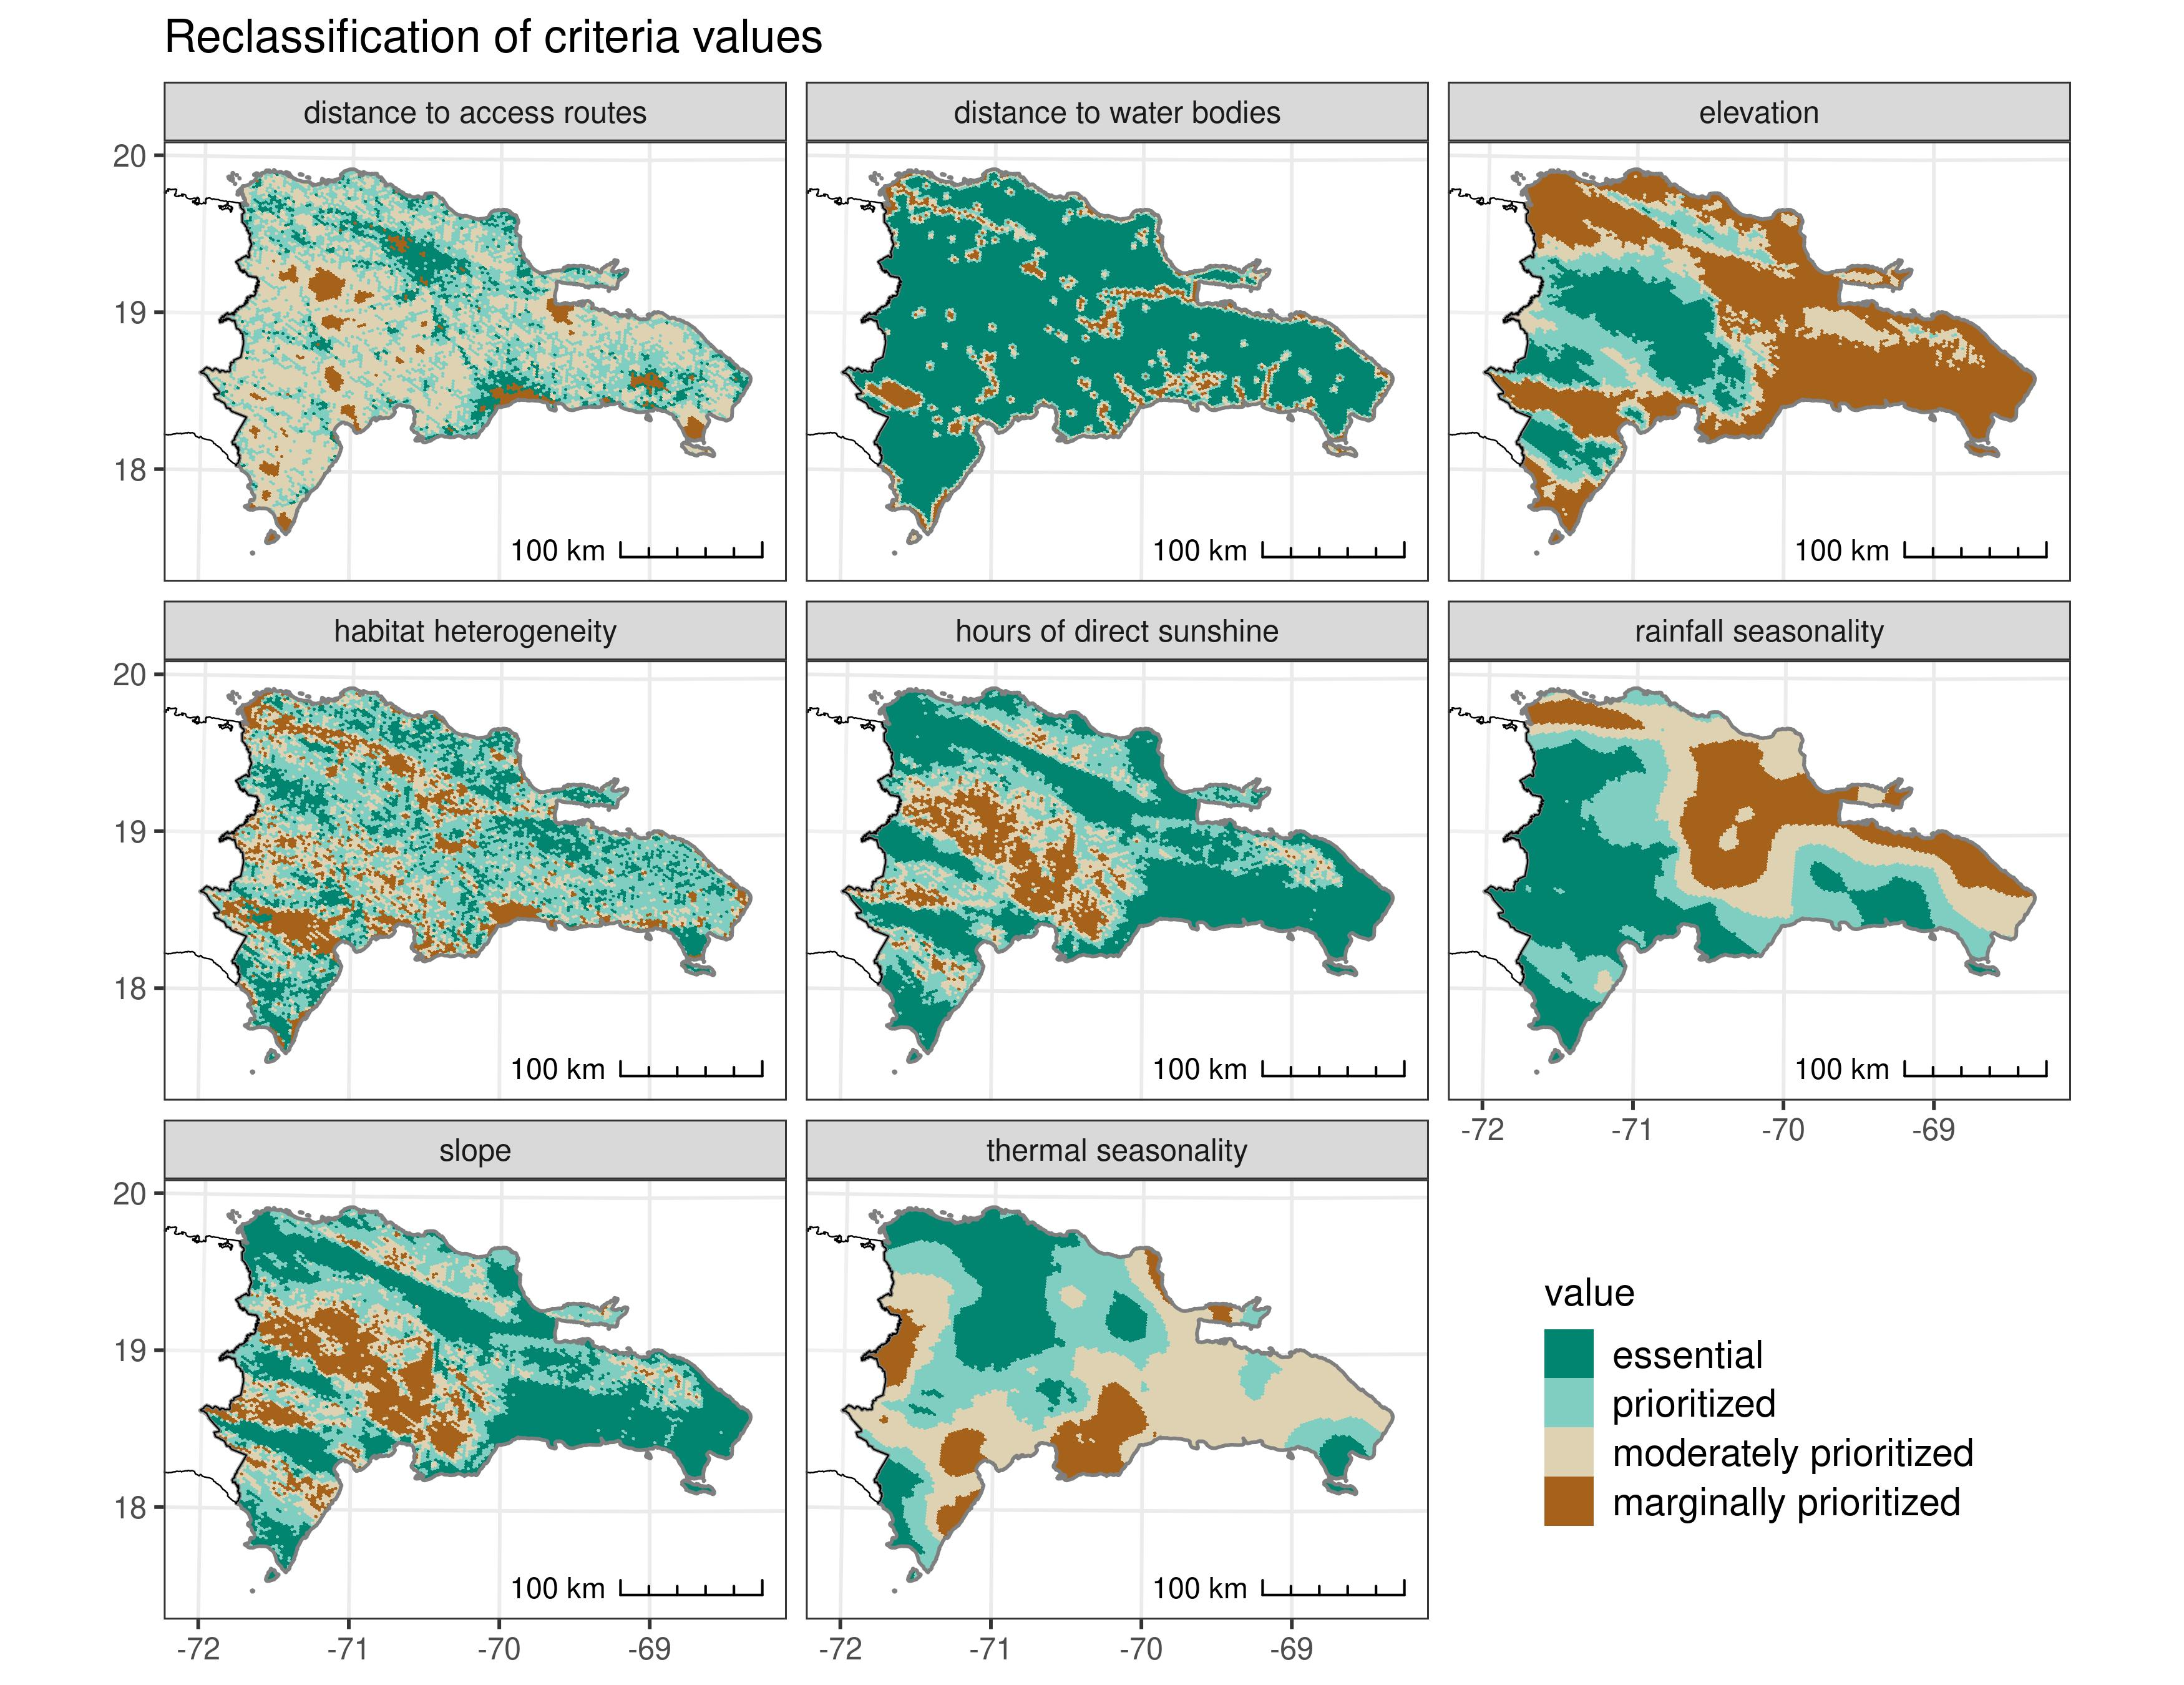
\includegraphics[width=1\linewidth]{figuras/all_criteria_mapa_eng_p} 

}

\caption{Reclassification of criteria values for weather station site selection across the Dominican Republic. Each panel represents the spatial distribution of priority categories (essential, prioritized, moderately prioritized, and marginally prioritized) for one of the evaluated criteria: distance to access routes, distance to water bodies, elevation, habitat heterogeneity, hours of direct sunshine, rainfall seasonality, slope, and thermal seasonality}\label{fig:all_criteria_mapa_eng_p}
\end{figure}

\begin{table}

\caption{\label{tab:puntuaciones_umbrales_eng}Thresholds used for reclassifying the average values of eight spatial criteria into four ordinal priority levels (essential, prioritized, moderately prioritized, and marginally prioritized) for weather station site selection in the Dominican Republic. Each row corresponds to a criterion, showing the intervals defined by the research team based on expert knowledge and bibliographic references.}
\centering
\begin{tabu} to \linewidth {m{4cm}m{2.6cm}m{2.6cm}m{2.6cm}m{2.6cm}}
\toprule
\textbf{Variable} & \textbf{Essential} & \textbf{Prioritized} & \textbf{Moderately prioritized} & \textbf{Marginally prioritized}\\
\midrule
distance to access routes & (50,200] & (200,500] & (500,5e+03] & {}[12.8,50] and (5e+03,3.28e+04]\\
thermal seasonality & (1.5,1.87] & (1.3,1.5] & (1.1,1.3] & {}[0.573,1.1]\\
rainfall seasonality & (50,89.6] & (40,50] & (30,40] & {}[19.5,30]\\
habitat heterogeneity & {}[0,300] & (300,450] & (450,600] & (600,3.56e+03]\\
distance to water bodies & (3e+03,2.64e+04] & (2e+03,3e+03] & (1e+03,2e+03] & {}[0,1e+03]\\
\addlinespace
slope & {}[0,3] & (3,9] & (9,15] & (15,32.7]\\
hours of direct sunshine & (4.3e+03,4.48e+03] & (4.1e+03,4.3e+03] & (3.9e+03,4.1e+03] & {}[3.18e+03,3.9e+03]\\
elevation & (800,2.79e+03] & (400,800] & (200,400] & {}[-42,200]\\
\bottomrule
\end{tabu}
\end{table}

We analyzed the reclassified scores for each criterion and observed wide
variability in the area covered by each priority category (see
Table~\ref{tab:proportionalareas}). Based on the AHP results, we
assigned high weights to rainfall and thermal seasonality, which
balanced the territory proportions relatively evenly across the four
priority classes. In contrast, we noticed that the criterion for hours
of direct sunshine led to a significant concentration of areas
classified as high-priority for establishing weather stations, including
``prioritized'' and ``essential''. Similarly, we identified numerous
hexagons categorized as ``prioritized'' and ``essential'' under the
elevation criterion. This result highlights how the Dominican Republic's
mountainous regions, with the lowest WS density, drove us to prioritize
elevated topography for establishing new stations.

\begin{table}

\caption{\label{tab:proportionalareas}Percentage of area by criteria used in the selection process for optimal weather station sites, emphasizing each criterion's contribution to the prioritization framework}
\centering
\begin{tabu} to \linewidth {m{4.4cm}>{\raggedleft\arraybackslash}p{2.2cm}>{\raggedleft\arraybackslash}p{2.2cm}>{\raggedleft\arraybackslash}p{2.2cm}>{\raggedleft\arraybackslash}p{2.2cm}>{\raggedleft}X}
\toprule
\textbf{Variable} & \textbf{Essential} & \textbf{Prioritized} & \textbf{Moderately prioritized} & \textbf{Marginally prioritized} & \textbf{Total}\\
\midrule
distance to access routes & 11.54 & 33.77 & 48.85 & 5.84 & 100\\
thermal seasonality & 22.17 & 28.11 & 38.39 & 11.33 & 100\\
rainfall seasonality & 33.90 & 22.95 & 21.67 & 21.47 & 100\\
habitat heterogeneity & 19.88 & 43.74 & 20.16 & 16.22 & 100\\
distance to water bodies & 75.04 & 8.04 & 8.72 & 8.20 & 100\\
\addlinespace
slope & 39.60 & 28.86 & 16.92 & 14.63 & 100\\
hours of direct sunshine & 48.23 & 25.06 & 16.03 & 10.68 & 100\\
elevation & 17.05 & 16.03 & 16.53 & 50.39 & 100\\
\bottomrule
\end{tabu}
\end{table}

We analyzed the distribution of aggregated categories before and after
applying exclusion based on limiting factors, highlighting key
differences in spatial coverage and proportional areas. Initially, the
aggregated categories without exclusions showed a dominance of
intermediate priorities, as moderately prioritized and prioritized
accounted for 70\% of the total studied area, while marginally
prioritized and essential shared the remaining 30\%
(Table~\ref{tab:areas_prop_all_criteria_con_sin_excl_eng}, second
column). These categories were spatially well distributed across the
Dominican Republic
(Figure~\ref{fig:all_criteria_scores_non_excluded_and_excluded_map_eng_p},
left), reflecting the AHP method's focus on prioritizing areas with
favorable environmental and geographical attributes. High-priority
hexagons (prioritized and essential) were mainly located in regions with
high seasonality, particularly in mountainous areas and along the
eastern edge of the country, which also exhibited good performance in
hours of sunshine. Conversely, hexagons categorized as marginally
prioritized were predominantly found in lower elevation areas with
limited sunshine hours, steep slopes, and low thermal and rainfall
seasonality.

After applying exclusion based on limiting factors, the distribution of
aggregated categories revealed significant changes in both spatial
patterns and proportional coverage. A total of 1508 hexagons were
assigned the category marginally prioritized due to their proximity to
water bodies, location within populated areas, or remoteness in terms of
accessibility. These excluded areas included inland and coastal lakes
and lagoons, coastal zones, wide rivers, reservoirs, and inaccessible
mountainous regions. As shown in
Figure~\ref{fig:all_criteria_scores_non_excluded_and_excluded_map_eng_p}
(right), the updated distribution reflects a refinement in
prioritization, ensuring that the remaining areas meet the necessary
conditions for weather station placement. The proportional areas of the
aggregated categories after exclusion are summarized in
Table~\ref{tab:areas_prop_all_criteria_con_sin_excl_eng} (third column),
highlighting a redistribution that prioritizes feasible and
representative locations for weather stations.

\begin{figure}[!ht]

{\centering 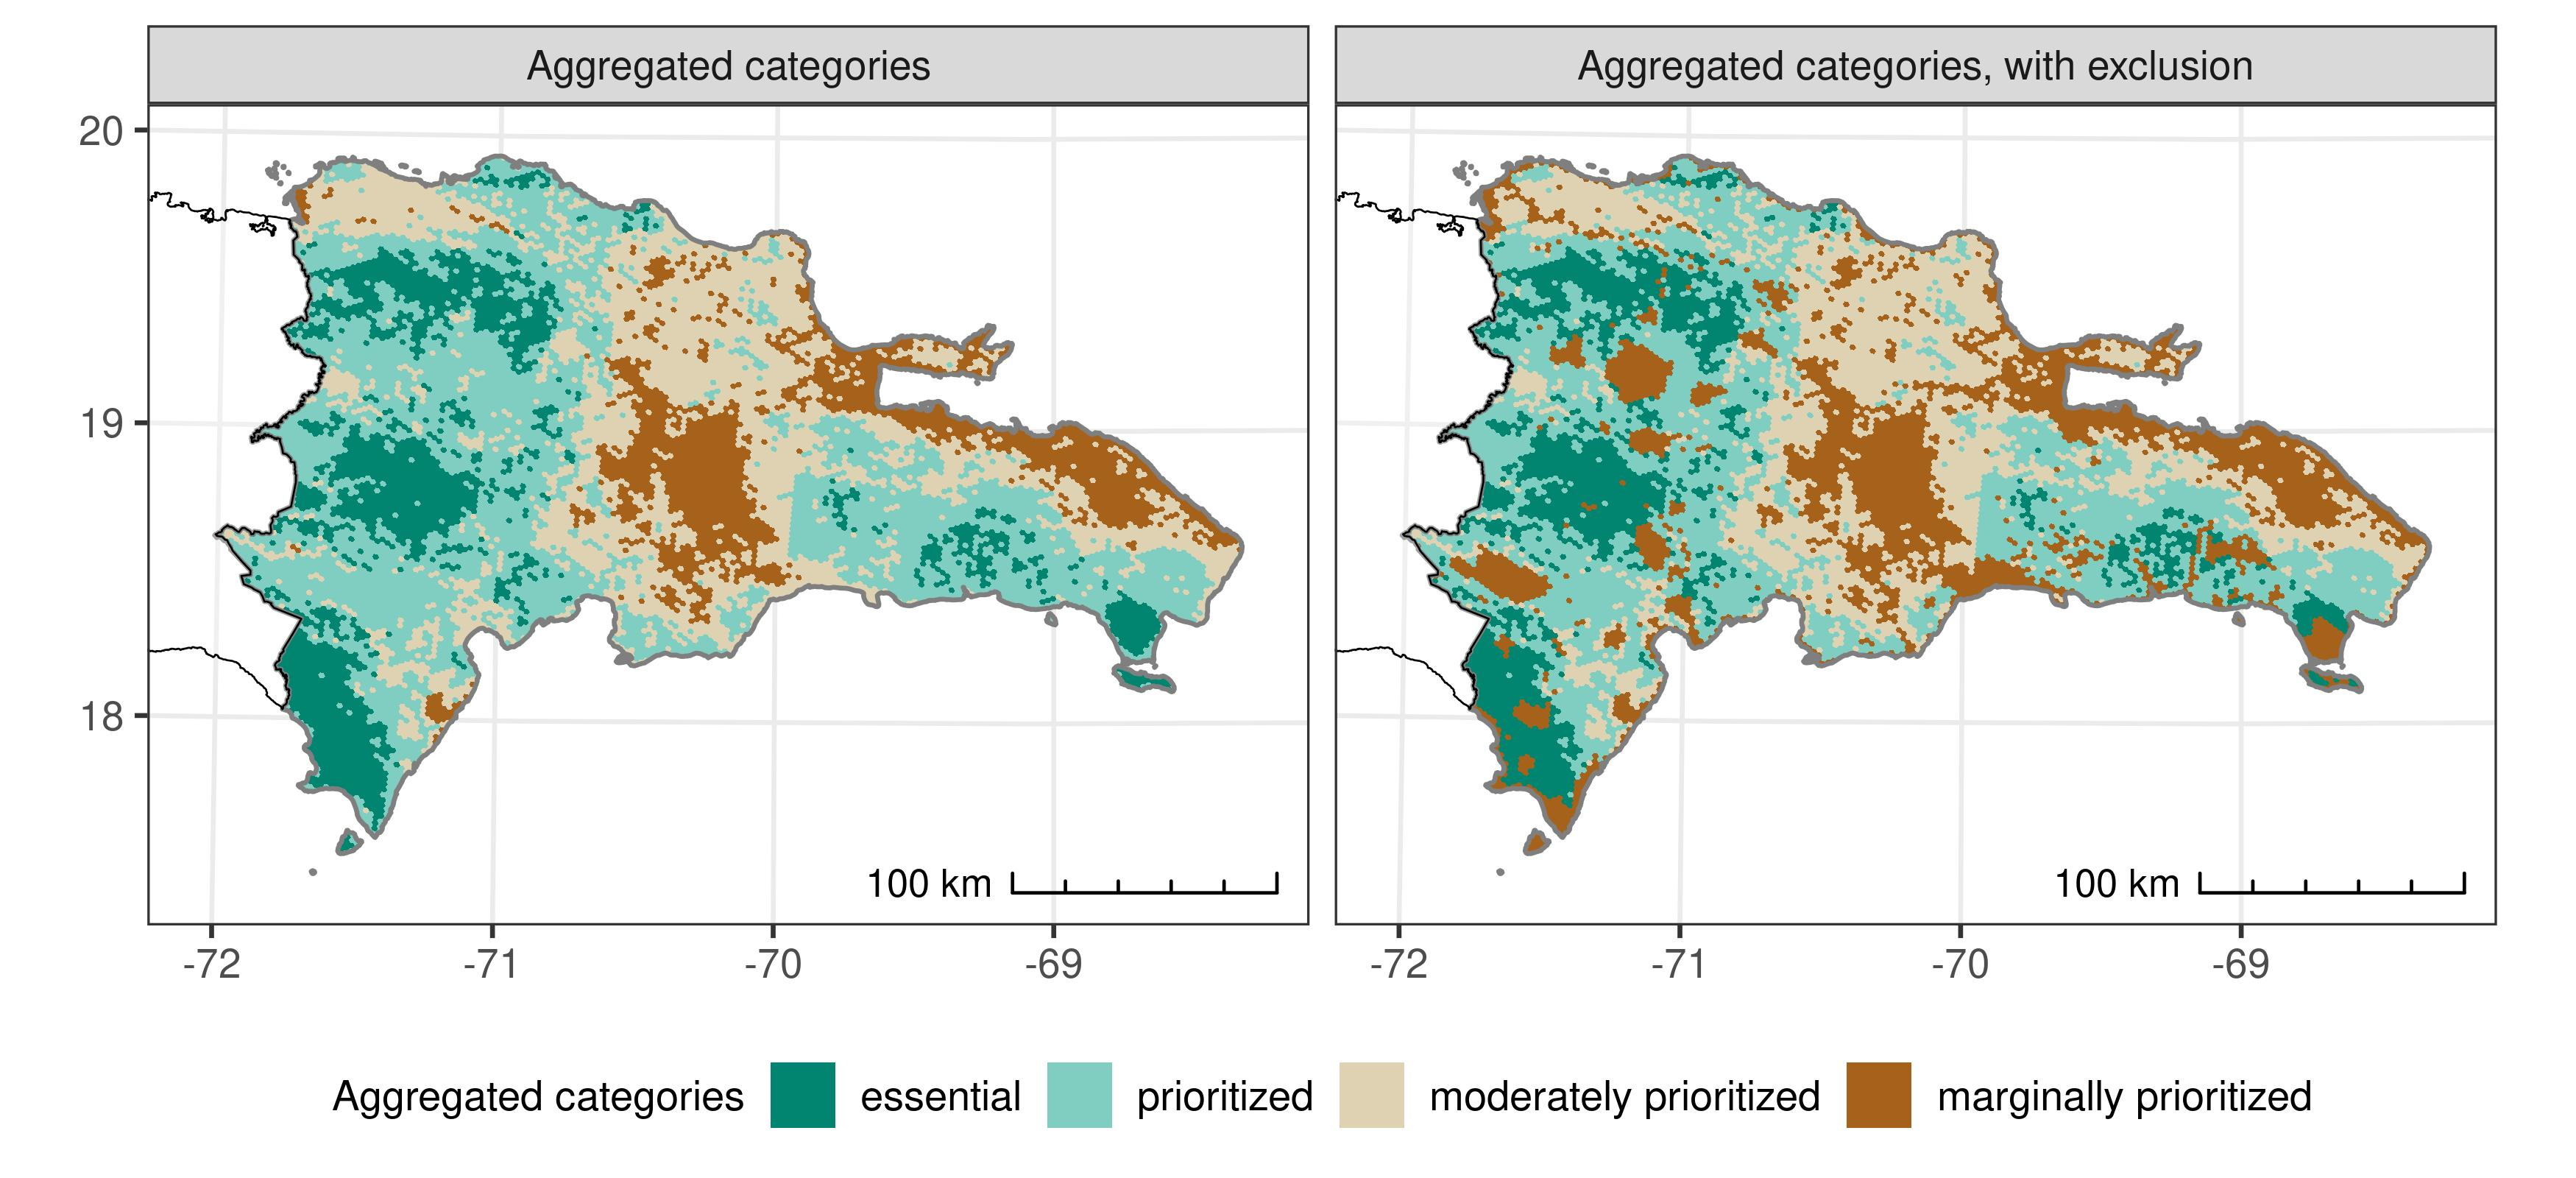
\includegraphics[width=1\linewidth]{figuras/all_criteria_scores_non_excluded_and_excluded_map_eng_p} 

}

\caption{Map of aggregated categories, with and without exclusion based on limiting factors}\label{fig:all_criteria_scores_non_excluded_and_excluded_map_eng_p}
\end{figure}

\begin{table}

\caption{\label{tab:areas_prop_all_criteria_con_sin_excl_eng}Percentage of area covered by aggregated categories for weather station site selection, with and without exclusion based on limiting factors}
\centering
\begin{tabu} to \linewidth {>{\raggedright\arraybackslash}p{3.8cm}>{\raggedleft\arraybackslash}p{5.5cm}>{\raggedleft\arraybackslash}p{5.5cm}}
\toprule
\textbf{Aggregated category} & \textbf{Without exclusion} & \textbf{With exclusion}\\
\midrule
Marginally prioritized & 13.79 & 24.08\\
Moderately prioritized & 30.81 & 26.95\\
Prioritized & 39.62 & 34.39\\
Essential & 15.77 & 14.59\\
Total & 100.00 & 100.00\\
\bottomrule
\end{tabu}
\end{table}

Our final step involved proposing site locations based on the priority
categories and criteria established in the earlier stages. These
proposals aim to address gaps in the existing weather station network by
suggesting new locations that meet the requirements of either essential
or prioritized. Using the refined spatial distribution after exclusions,
we generated three scenarios with varying station densities: 100, 150,
and 250~km\textsuperscript{2} per station. Each scenario represents an
optimized distribution of proposed sites, tailored to achieve
comprehensive spatial coverage while considering practical constraints
and priorities.

In the first scenario
(Figure~\ref{fig:esc_100_150_250_activas_buenas_mapa_eng},~top), where
each station covers 100~km\textsuperscript{2} of area, we recommend the
installation of 170 new stations. The map clearly distinguishes the
proposed sites categorized as ``prioritized'' and ``essential''. The
proposed ``essential'' sites are predominantly concentrated in the
central and eastern regions of the Dominican Republic, particularly
along mountainous areas and regions with higher elevation. In contrast,
``prioritized'' sites show a broader distribution, extending into the
northern and southern regions, covering a mix of coastal areas and
lowlands. Notably, the southern coastal plains, lowlands, and
mid-altitude regions feature a higher proportion of prioritized sites,
highlighting the emphasis on coverage in areas with fewer terrain and
environmental constraints. In the northeast and central DR, proposed
sites are scattered, with a focus on bridging gaps in spatial coverage
in flatter, lower-priority regions.

Expanding on the analysis, the second scenario
(Figure~\ref{fig:esc_100_150_250_activas_buenas_mapa_eng},~middle)
assumed a coverage of 150~km\textsuperscript{2} per station. We followed
a similar process and recommended installing 89 new stations. The map
distinguished the proposed sites categorized as ``prioritized'' and
``essential'', and showed how the spatial distribution shifted notably
compared to the first scenario. Our proposal concentrated ``essential''
sites in the central and western regions, particularly in mountainous
areas and regions with complex terrain, though their density decreased
slightly due to the existing broader station coverage in the east
region. In contrast, ``prioritized'' sites spread more evenly across the
country, with a marked presence in valleys and plains. This scenario
demonstrated our effort to balance the inclusion of essential and
prioritized areas while maintaining a cohesive spatial configuration.
Additionally, we extended coverage into areas less emphasized in the
first scenario, particularly along the central valleys and northern
slopes, further bridging gaps in the network.

\begin{figure}[!ht]

{\centering 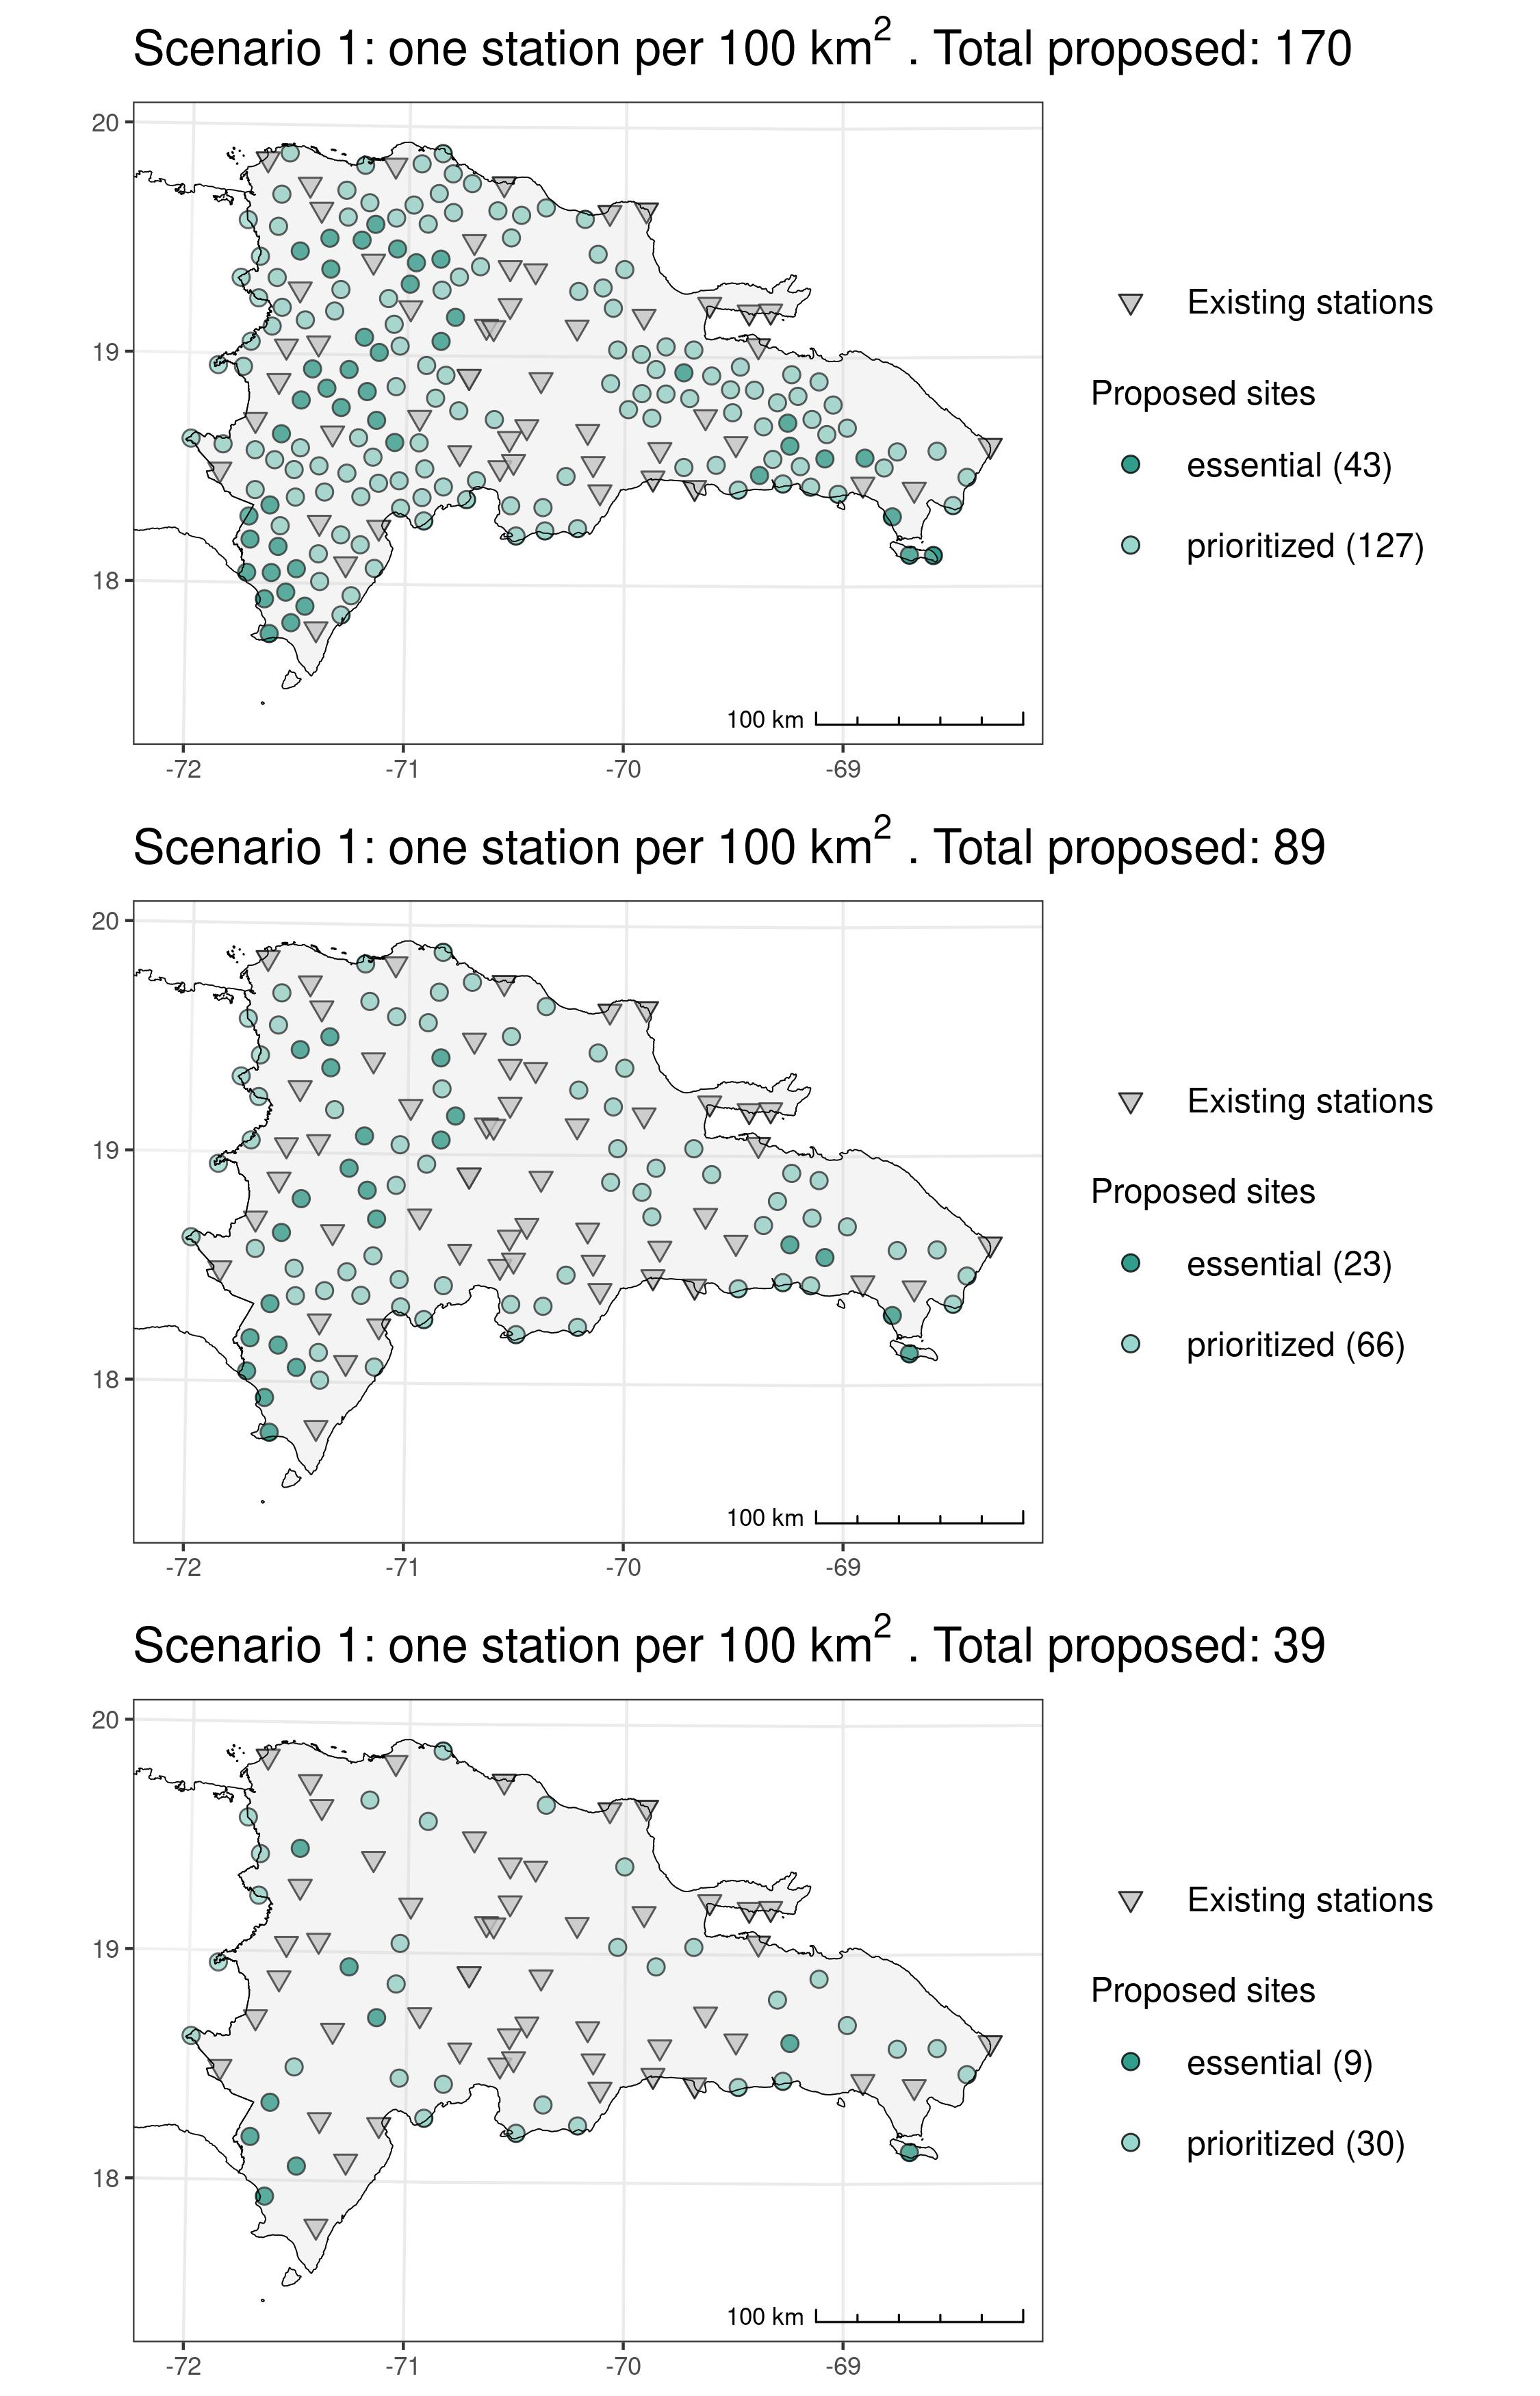
\includegraphics[width=0.7\linewidth]{figuras/esc_100_150_250_activas_buenas_mapa_eng} 

}

\caption{Spatial distribution of existing and proposed weather stations (WS) under three different scenarios of station density in the Dominican Republic: one station per 100 km\textsuperscript{2} (top), 150 km\textsuperscript{2} (middle), and 250 km\textsuperscript{2} (bottom). Existing stations are represented by inverted triangles, while proposed sites are represented by circles. The proposed sites are classified into two categories: "essential" and "prioritized," with their respective counts shown in the legend. Proposed sites have been selected to avoid redundancy with existing stations in "Good or Active" condition managed by INDOMET and INDRHI}\label{fig:esc_100_150_250_activas_buenas_mapa_eng}
\end{figure}

In the third scenario, with a coverage of 250~km\textsuperscript{2} per
station, we recommended installing 39 new stations
(Figure~\ref{fig:esc_100_150_250_activas_buenas_mapa_eng},~bottom). The
resulting map emphasizes the focus on maximizing coverage in priority
areas while ensuring efficient resource allocation. Proposed sites in
``essential'' areas were primarily located in the central and western
regions, continuing the pattern observed in previous scenarios. However,
their distribution became more dispersed due to the lower station
density. On the other hand, ``prioritized'' dominated across the
country, particularly in areas where terrain and environmental
constraints are less severe. This scenario also extended coverage to
underrepresented regions in the northwest, filling significant gaps in
the spatial distribution. The broader spacing of stations in this
scenario highlights the trade-offs involved in balancing territorial
coverage, resource efficiency, and budget constraints.

\hypertarget{discussion}{%
\section{Discussion}\label{discussion}}

We successfully achieved the primary objectives of this study by
integrating geospatial analysis with the Analytic Hierarchy Process
(AHP) to propose optimal site locations for weather stations (WS) in the
Dominican Republic. This approach allowed us to systematically address
gaps in the existing network and align new site proposals with
environmental, accessibility, and governance priorities (Izzo et al.,
2010; Programa Mundial de Alimentos (PMA), 2019).

The results demonstrate the value of combining multi-criteria
decision-making (MCDM) methods with neighborhood analysis for spatial
planning. Key findings include the identification of high-priority areas
based on thermal and rainfall seasonality, elevation, and solar
radiation, which collectively emphasize the importance of elevated
regions with significant climatic variability (Izzo et al., 2010; Rojas
Briceño et al., 2021). These results align with previous studies
highlighting the role of these variables in optimizing WS placement, but
our study advances the field by explicitly incorporating redundancy
constraints through a neighborhood-based exclusion process using a
custom-developed function.

Our methodological approach offers several innovations compared to
previous studies. First, the use of the H3 hexagonal indexing system
enhanced the spatial resolution and computational efficiency of zonal
statistics. Second, the integration of geospatial tools like Google
Earth Engine (GEE) with AHP allowed us to streamline the workflow,
facilitating the prioritization of thousands of candidate sites across
the Dominican Republic. Third, the disaggregation of proposed sites into
``essential'' and ``prioritize'' categories introduces a flexible
framework for decision-makers to allocate resources according to budget
constraints and governance structures.

The scenarios generated for station densities---100, 150, and
250,km\textsuperscript{2} per station---provide practical pathways for
WS network expansion, while simultaneously adhering to the
recommendations of national and international entities (Programa Mundial
de Alimentos (PMA), 2019; World Meteorological Organization (WMO) \& The
International Association of Hydrological Sciences, 1976). Each scenario
reflects trade-offs between spatial coverage and resource efficiency,
offering stakeholders the flexibility to adapt the recommendations to
evolving priorities. Notably, our results show that higher-density
scenarios (e.g., 100,km\textsuperscript{2}) achieve comprehensive
coverage in critical areas, while lower-density scenarios (e.g.,
250,km\textsuperscript{2}) maintain representativeness with reduced
resource investment.

Despite these strengths, several limitations should be acknowledged.
While the proposed site locations are based on robust spatial analysis,
the definitive selection of WS locations requires field validation to
assess terrain constraints, local accessibility, and potential land-use
conflicts. Additionally, the study's exclusion criteria focused
primarily on proximity to water bodies and existing WS networks but did
not account for other potential barriers, such as detailed accessibility
constraints or issues related to land ownership. These factors
underscore the need for complementary qualitative assessments during
implementation.

Our approach also highlights opportunities for leveraging DIY and
low-cost equipment in expanding WS networks, particularly in a global
context where high-density data and microclimate information are
increasingly demanded for specific studies (Chan et al., 2021; Theisen
et al., 2020). These solutions are particularly relevant for deploying
stations in prioritized areas, as they can reduce costs while
maintaining sufficient data quality for certain applications (Kemppinen
et al., 2024). Furthermore, integrating educational initiatives with WS
deployment---such as collaborating with schools and community
organizations---can enhance the sustainability and societal impact of
these networks.

In conclusion, this study provides a replicable framework for WS network
planning that combines advanced geospatial analysis with expert-driven
criteria prioritization. The proposed methodology is not only relevant
for the Dominican Republic but also adaptable to other regions facing
similar challenges in optimizing WS networks. Future research should
explore the integration of additional environmental variables, such as
wind patterns or soil characteristics, and evaluate the long-term
performance of deployed WS in capturing climatic variability. By
addressing these avenues, stakeholders can further enhance the
resilience and functionality of WS networks in the face of evolving
climatic and societal demands.

\hypertarget{conflict-of-interest-declaration}{%
\section*{Conflict of Interest
Declaration}\label{conflict-of-interest-declaration}}
\addcontentsline{toc}{section}{Conflict of Interest Declaration}

The authors declare that they have no conflict of interest related to
the content of this article.

\hypertarget{author-contributions}{%
\section{Author Contributions}\label{author-contributions}}

JM and MI conceptualized and designed the study. JM was responsible for
data collection. JM and MI established the methodology and conducted the
research. JM developed the software, and supervision was carried out by
MI. Both validated the work. JM and MI were in charge of visualization
and drafted the original manuscript.

\hypertarget{data-scripts-and-code-availability}{%
\section*{Data, Scripts, and Code
Availability}\label{data-scripts-and-code-availability}}
\addcontentsline{toc}{section}{Data, Scripts, and Code Availability}

The data supporting the findings of this study are openly available on
Zenodo at \url{} {[}{]}. The scripts used for data curation, analysis,
and visualization are available in this section, as well as in the
GitHub repository at
\url{https://github.com/geofis/seleccion-sitios-estaciones-meteoclimaticas-rd}
and here
\url{https://github.com/geofis/datos-meteoclimaticos-escenarios-cc}, and
on Zenodo at \url{} {[}{]}.

\newpage

\hypertarget{references}{%
\section*{References}\label{references}}
\addcontentsline{toc}{section}{References}

\hypertarget{refs}{}
\begin{CSLReferences}{1}{0}
\leavevmode\vadjust pre{\hypertarget{ref-ali2018}{}}%
Ali, M. Z. M., \& Othman, F. (2018). Raingauge network optimization in a
tropical urban area by coupling cross-validation with the geostatistical
technique. \emph{Hydrological Sciences Journal}, \emph{63}(3), 474--491.
\url{https://doi.org/10.1080/02626667.2018.1437271}

\leavevmode\vadjust pre{\hypertarget{ref-bertini2021}{}}%
Bertini, C., Ridolfi, E., de Padua, L. H. R., Russo, F., Napolitano, F.,
\& Alfonso, L. (2021). An entropy-based approach for the optimization of
rain gauge network using satellite and ground-based data.
\emph{Hydrology Research}, \emph{52}(3), 620--635.
\url{https://doi.org/10.2166/nh.2021.113}

\leavevmode\vadjust pre{\hypertarget{ref-chakhar2008spatial}{}}%
Chakhar, S., \& Mousseau, V. (2008). Spatial multicriteria decision
making. \emph{Encyclopedia of GIS}, \emph{10}, 978--970.

\leavevmode\vadjust pre{\hypertarget{ref-kristofer2021low}{}}%
Chan, K., Schillereff, D. N., Baas, A. C., Chadwick, M. A., Main, B.,
Mulligan, M., O'Shea, F. T., Pearce, R., Smith, T. E., Soesbergen, A.
van, Tebbs, E., \& Thompson, J. (2021). Low-cost electronic sensors for
environmental research: Pitfalls and opportunities. \emph{Progress in
Physical Geography: Earth and Environment}, \emph{45}(3), 305--338.
\url{https://doi.org/10.1177/0309133320956567}

\leavevmode\vadjust pre{\hypertarget{ref-cho2019ahpsurvey}{}}%
Cho, F. (2019). \emph{Ahpsurvey: Analytic hierarchy process for survey
data}. \url{https://CRAN.R-project.org/package=ahpsurvey}

\leavevmode\vadjust pre{\hypertarget{ref-Chung2018SpatialAO}{}}%
Chung, W., Abdel-Aty, M. A., \& Lee, J. (2018). Spatial analysis of the
effective coverage of land-based weather stations for traffic crashes.
\emph{Applied Geography}, \emph{90}, 17--27.

\leavevmode\vadjust pre{\hypertarget{ref-eastman1998multi}{}}%
Eastman, J. R., Jiang, H., \& Toledano, J. (1998). Multi-criteria and
multi-objective decision making for land allocation using GIS.
\emph{Multicriteria Analysis for Land-Use Management}, 227--251.

\leavevmode\vadjust pre{\hypertarget{ref-frei2003designing}{}}%
Frei, T. (2003). Designing meteorological networks for switzerland
according to user requirements. \emph{Meteorological Applications},
\emph{10}(4), 313--317.

\leavevmode\vadjust pre{\hypertarget{ref-getodk2024}{}}%
Get ODK Inc. (2024). \emph{Get ODK}. \url{https://getodk.org/}.

\leavevmode\vadjust pre{\hypertarget{ref-google2023earthengine}{}}%
Google Earth Engine Contributors. (2023). \emph{Earth engine API}.
\url{https://github.com/google/earthengine-api}

\leavevmode\vadjust pre{\hypertarget{ref-GORELICK201718}{}}%
Gorelick, N., Hancher, M., Dixon, M., Ilyushchenko, S., Thau, D., \&
Moore, R. (2017). Google earth engine: Planetary-scale geospatial
analysis for everyone. \emph{Remote Sensing of Environment}, \emph{202},
18--27. https://doi.org/\url{https://doi.org/10.1016/j.rse.2017.06.031}

\leavevmode\vadjust pre{\hypertarget{ref-hartung2010odk}{}}%
Hartung, C., Lerer, A., Anokwa, Y., Tseng, C., Brunette, W., \&
Borriello, G. (2010). \emph{Open data kit: Tools to build information
services for developing regions}.
\url{https://doi.org/10.1145/2369220.2369236}

\leavevmode\vadjust pre{\hypertarget{ref-hijmans2023raster}{}}%
Hijmans, R. J. (2023). \emph{Raster: Geographic data analysis and
modeling}. \url{https://CRAN.R-project.org/package=raster}

\leavevmode\vadjust pre{\hypertarget{ref-hijmans2024terra}{}}%
Hijmans, R. J. (2024). \emph{Terra: Spatial data analysis}.
\url{https://CRAN.R-project.org/package=terra}

\leavevmode\vadjust pre{\hypertarget{ref-Izzo2010ANC}{}}%
Izzo, M., Rosskopf, C. M., Aucelli, P. P. C., Maratea, A., Méndez, R.
E., Pérez, C., \& Segura, H. (2010). {A New Climatic Map of the
Dominican Republic Based on the Thornthwaite Classification}.
\emph{Physical Geography}, \emph{31}, 455--472.

\leavevmode\vadjust pre{\hypertarget{ref-kemppinen_microclimate_2024}{}}%
Kemppinen, J., Lembrechts, J. J., Van Meerbeek, K., Carnicer, J.,
Chardon, N. I., Kardol, P., Lenoir, J., Liu, D., Maclean, I., Pergl, J.,
Saccone, P., Senior, R. A., Shen, T., Słowińska, S., Vandvik, V., Oppen,
J. von, Aalto, J., Ayalew, B., Bates, O., \ldots{} De Frenne, P. (2024).
Microclimate, an important part of ecology and biogeography.
\emph{Global Ecology and Biogeography}, \emph{33}(6), e13834.
\url{https://doi.org/10.1111/geb.13834}

\leavevmode\vadjust pre{\hypertarget{ref-koksalan2011multiple}{}}%
Köksalan, M. M., Wallenius, J., \& Zionts, S. (2011). \emph{Multiple
criteria decision making: From early history to the 21st century}. World
Scientific. \url{https://books.google.com.do/books?id=LqAw1539l/_cC}

\leavevmode\vadjust pre{\hypertarget{ref-LincolnLenderking2020ClimateCA}{}}%
Lincoln Lenderking, H., Robinson, S., \& Carlson, G. R. (2020). {Climate
change and food security in Caribbean small island developing states:
challenges and strategies}. \emph{International Journal of Sustainable
Development \& World Ecology}, \emph{28}, 238--245.

\leavevmode\vadjust pre{\hypertarget{ref-Lohmann2016ComparingVA}{}}%
Lohmann, H. (2016). {Comparing vulnerability and adaptive capacity to
climate change in individuals of coastal Dominican Republic}.
\emph{Ocean \& Coastal Management}, \emph{132}, 111--119.

\leavevmode\vadjust pre{\hypertarget{ref-Mackay2017TheFO}{}}%
Mackay, E. A., \& Spencer, A. J. (2017). {The future of Caribbean
tourism: competition and climate change implications}. \emph{Worldwide
Hospitality and Tourism Themes}, \emph{9}, 44--59.

\leavevmode\vadjust pre{\hypertarget{ref-malczewski2004gis}{}}%
Malczewski, J. (2004). GIS-based land-use suitability analysis: A
critical overview. \emph{Progress in Planning}, \emph{62}(1), 3--65.

\leavevmode\vadjust pre{\hypertarget{ref-Marchi2019EvaluatingWV}{}}%
Marchi, M., Sinjur, I., Bozzano, M., \& Westergren, M. (2019).
Evaluating WorldClim version 1 (1961--1990) as the baseline for
sustainable use of forest and environmental resources in a changing
climate. \emph{Sustainability}.

\leavevmode\vadjust pre{\hypertarget{ref-jose_ramon_martinez_batlle_2022_7367180}{}}%
Martínez-Batlle, J. R. (2022). \emph{{Estadística zonal multipropósito
sobre información geoespacial de República Dominicana, usando Google
Earth Engine, Python y R}} (Version v0.0.0.9000) {[}Computer
software{]}. Zenodo. \url{https://doi.org/10.5281/zenodo.7367256}

\leavevmode\vadjust pre{\hypertarget{ref-Le2019ClimateCA}{}}%
Ngoc Le, T. D. (2019). Climate change adaptation in coastal cities of
developing countries: Characterizing types of vulnerability and
adaptation options. \emph{Mitigation and Adaptation Strategies for
Global Change}, \emph{25}, 739--761.

\leavevmode\vadjust pre{\hypertarget{ref-pebesma2018simple}{}}%
Pebesma, E. (2018). {Simple Features for R: Standardized Support for
Spatial Vector Data}. \emph{{The R Journal}}, \emph{10}(1), 439--446.
\url{https://doi.org/10.32614/RJ-2018-009}

\leavevmode\vadjust pre{\hypertarget{ref-pebesma2023spatial}{}}%
Pebesma, E., \& Bivand, R. (2023). \emph{{Spatial Data Science: With
applications in R}}. {Chapman and Hall/CRC}.
\url{https://doi.org/10.1201/9780429459016}

\leavevmode\vadjust pre{\hypertarget{ref-pebesma2016measurement}{}}%
Pebesma, E., Mailund, T., \& Hiebert, J. (2016). Measurement units in
{R}. \emph{R Journal}, \emph{8}(2), 486--494.
\url{https://doi.org/10.32614/RJ-2016-061}

\leavevmode\vadjust pre{\hypertarget{ref-proyecto2019pma}{}}%
Programa Mundial de Alimentos (PMA). (2019). \emph{{Proyecto Resiliencia
a la Sequía. Fortalecimiento de capacidades para mejorar la seguridad
alimentaria y la resiliencia ante sequía en Haití y la República
Dominicana. Proyecto de preparación ante emergencias basado en
pronósticos de riesgos climáticos en República Dominicana (FBF)}}.
{Programa Mundial de Alimentos (PMA)}.

\leavevmode\vadjust pre{\hypertarget{ref-rcoreteam2024r}{}}%
R Core Team. (2024). \emph{R: A language and environment for statistical
computing}. R Foundation for Statistical Computing.
\url{https://www.R-project.org/}

\leavevmode\vadjust pre{\hypertarget{ref-rojasbriceno2021}{}}%
Rojas Briceño, N. B., Salas López, R., Silva López, J. O., Oliva-Cruz,
M., Gómez Fernández, D., Terrones Murga, R. E., Iliquín Trigoso, D.,
Barrena Gurbillón, M., \& Barboza, E. (2021). Site Selection for a
Network of Weather Stations Using AHP and Near Analysis in a GIS
Environment in Amazonas, NW Peru. \emph{Climate}, \emph{9}(12), 169.
\url{https://doi.org/10.3390/cli9120169}

\leavevmode\vadjust pre{\hypertarget{ref-Roson2013AMF}{}}%
Roson, R. (2013). {A Modeling Framework to Assess the Economic Impact of
Climate Change in the Caribbean}. \emph{Cepal Review}, \emph{111},
23--36.

\leavevmode\vadjust pre{\hypertarget{ref-saaty1977}{}}%
Saaty, T. L. (1977). A scaling method for priorities in hierarchical
structures. \emph{Journal of Mathematical Psychology}, \emph{15}(3),
234--281. \url{https://doi.org/10.1016/0022-2496(77)90033-5}

\leavevmode\vadjust pre{\hypertarget{ref-saaty2001}{}}%
Saaty, T. L. (2001). \emph{Fundamentals of the Analytic Hierarchy
Process} (D. L. Schmoldt, J. Kangas, G. A. Mendoza, \& M. Pesonen, Eds.;
Vol. 3, pp. 15--35). Springer Netherlands.
\url{http://link.springer.com/10.1007/978-94-015-9799-9_2}

\leavevmode\vadjust pre{\hypertarget{ref-saaty2013}{}}%
Saaty, T. L. (2013). The Modern Science of Multicriteria Decision Making
and Its Practical Applications: The AHP/ANP Approach. \emph{Operations
Research}, \emph{61}(5), 1101--1118.
\url{https://doi.org/10.1287/opre.2013.1197}

\leavevmode\vadjust pre{\hypertarget{ref-saaty2007}{}}%
Saaty, T. L., \& Tran, L. T. (2007). On the invalidity of fuzzifying
numerical judgments in the Analytic Hierarchy Process.
\emph{Mathematical and Computer Modelling}, \emph{46}(7-8), 962--975.
\url{https://doi.org/10.1016/j.mcm.2007.03.022}

\leavevmode\vadjust pre{\hypertarget{ref-safavi2021}{}}%
Safavi, M., Siuki, A. K., \& Hashemi, S. R. (2021). New optimization
methods for designing rain stations network using new neural network,
election, and whale optimization algorithms by combining the Kriging
method. \emph{Environmental Monitoring and Assessment}, \emph{193}(1),
4. \url{https://doi.org/10.1007/s10661-020-08726-z}

\leavevmode\vadjust pre{\hypertarget{ref-encyclopedia3010006}{}}%
Taherdoost, H., \& Madanchian, M. (2023). Multi-criteria decision making
(MCDM) methods and concepts. \emph{Encyclopedia}, \emph{3}(1), 77--87.
\url{https://doi.org/10.3390/encyclopedia3010006}

\leavevmode\vadjust pre{\hypertarget{ref-tekleyohannes2021}{}}%
Tekleyohannes, M., Grum, B., Abebe, N., \& Abebe, B. A. (2021).
Optimization of rain gauge network using multi-criteria decision
analysis and entropy approaches: case of Tekeze River basin,
northwestern Ethiopia. \emph{Theoretical and Applied Climatology},
\emph{145}(1-2), 159--174.
\url{https://doi.org/10.1007/s00704-021-03604-1}

\leavevmode\vadjust pre{\hypertarget{ref-theisen2020more}{}}%
Theisen, A., Ungar, M., Sheridan, B., \& Illston, B. G. (2020). More
science with less: Evaluation of a 3D-printed weather station.
\emph{Atmospheric Measurement Techniques}, \emph{13}(9), 4699--4713.
\url{https://doi.org/10.5194/amt-13-4699-2020}

\leavevmode\vadjust pre{\hypertarget{ref-theochari2021hydrometeorological}{}}%
Theochari, A.-P., Feloni, E., Bournas, A., \& Baltas, E. (2021).
Hydrometeorological-hydrometric station network design using
multicriteria decision analysis and GIS techniques. \emph{Environmental
Processes}, \emph{8}, 1099--1119.

\leavevmode\vadjust pre{\hypertarget{ref-thiriez1975multiple}{}}%
Thiriez, H., \& Zionts, S. (1975). \emph{Multiple criteria decision
making: Proceedings of a conference jouy-en-josas, france may 21--23,
1975} (Vol. 130). Springer Science \& Business Media.

\leavevmode\vadjust pre{\hypertarget{ref-uber2024h3}{}}%
Uber Technologies, Inc. (2024). \emph{{H3. Hierarchical Hexagonal
Geospatial Indexing System}}. Available online:
\url{https://h3geo.org/docs} (accessed December, 2024).

\leavevmode\vadjust pre{\hypertarget{ref-valipour2019}{}}%
Valipour, E., Ghorbani, M. A., \& Asadi, E. (2019). Evaluation and
Optimization of Rain Gauge Network Based on the Geostatistic Methods and
Firefly Algorithm. (Case study: Eastern Basin of Urmia Lake).
\emph{Irrigation Sciences and Engineering}, \emph{42}(4), 153--166.
\url{https://doi.org/10.22055/jise.2018.20549.1477}

\leavevmode\vadjust pre{\hypertarget{ref-hadley2019welcome}{}}%
Wickham, H., Averick, M., Bryan, J., Chang, W., McGowan, L. D.,
François, R., Grolemund, G., Hayes, A., Henry, L., Hester, J., Kuhn, M.,
Pedersen, T. L., Miller, E., Bache, S. M., Müller, K., Ooms, J.,
Robinson, D., Seidel, D. P., Spinu, V., \ldots{} Yutani, H. (2019).
Welcome to the {tidyverse}. \emph{Journal of Open Source Software},
\emph{4}(43), 1686. \url{https://doi.org/10.21105/joss.01686}

\leavevmode\vadjust pre{\hypertarget{ref-vanWilgen2016RisingTA}{}}%
Wilgen, N. J. van, Goodall, V. L., Holness, S. D., Chown, S. L., \&
McGeoch, M. A. (2016). Rising temperatures and changing rainfall
patterns in south africa's national parks. \emph{International Journal
of Climatology}, \emph{36}.

\leavevmode\vadjust pre{\hypertarget{ref-world1996guia}{}}%
World Meteorological Organization (WMO). (1996). \emph{Guía de
instrumentos y métodos de observación meteorológicos}. Secretaría de la
Organización Meteorológica Mundial.

\leavevmode\vadjust pre{\hypertarget{ref-wmo2017guia}{}}%
World Meteorological Organization (WMO). (2017a). \emph{Guía de
instrumentos y métodos de observación meteorológicos}. World
Meteorological Organization Geneva, Switzerland.

\leavevmode\vadjust pre{\hypertarget{ref-wmo2017guide}{}}%
World Meteorological Organization (WMO). (2017b). \emph{Guide to the WMO
integrated global observing system. WMO-no. 1165}. World Meteorological
Organization, Geneva, Switzerland.

\leavevmode\vadjust pre{\hypertarget{ref-wmo2020guide}{}}%
World Meteorological Organization (WMO). (2020). \emph{Guide to
hydrological practices. Volume i: Hydrology---from measurement to
hydrological information. WMO report no. 168} (p. 296). World
Meteorological Organization, Geneva, Switzerland.

\leavevmode\vadjust pre{\hypertarget{ref-design1976hydrological}{}}%
World Meteorological Organization (WMO), \& The International
Association of Hydrological Sciences. (1976). \emph{Hydrological network
design and information transfer}. {Secretariat of the World
Meteorological Organization}.

\leavevmode\vadjust pre{\hypertarget{ref-wu_geemap_2020}{}}%
Wu, Q. (2020). Geemap: {A} {Python} package for interactive mapping with
{Google} {Earth} {Engine}. \emph{Journal of Open Source Software},
\emph{5}(51), 2305. \url{https://doi.org/10.21105/joss.02305}

\leavevmode\vadjust pre{\hypertarget{ref-xie2014implementing}{}}%
Xie, Y. (2014). Knitr: A comprehensive tool for reproducible research in
{R}. In V. Stodden, F. Leisch, \& R. D. Peng (Eds.), \emph{Implementing
reproducible computational research}. Chapman; Hall/CRC.

\leavevmode\vadjust pre{\hypertarget{ref-xie2020rmarkdown}{}}%
Xie, Y., Dervieux, C., \& Riederer, E. (2020). \emph{R markdown
cookbook}. Chapman; Hall/CRC.
\url{https://bookdown.org/yihui/rmarkdown-cookbook}

\leavevmode\vadjust pre{\hypertarget{ref-zhu2021kableextra}{}}%
Zhu, H. (2021). \emph{kableExtra: Construct complex table with 'kable'
and pipe syntax}. \url{https://CRAN.R-project.org/package=kableExtra}

\end{CSLReferences}

\bibliographystyle{unsrt}
\bibliography{references.bib}


\end{document}
